\documentclass{beamer}
\mode<presentation>
\usepackage{amsmath}
\usepackage{amssymb}
%\usepackage{advdate}
\usepackage{adjustbox}
\usepackage{subcaption}
\usepackage{enumitem}
\usepackage{multicol}
\usepackage{mathtools}
\usepackage{listings}
\usepackage{url}
\def\UrlBreaks{\do\/\do-}
\usetheme{Boadilla}
\usecolortheme{lily}
\setbeamertemplate{footline}
{
  \leavevmode%
  \hbox{%
  \begin{beamercolorbox}[wd=\paperwidth,ht=2.25ex,dp=1ex,right]{author in head/foot}%
    \insertframenumber{} / \inserttotalframenumber\hspace*{2ex} 
  \end{beamercolorbox}}%
  \vskip0pt%
}
\setbeamertemplate{navigation symbols}{}

\providecommand{\nCr}[2]{\,^{#1}C_{#2}} % nCr
\providecommand{\nPr}[2]{\,^{#1}P_{#2}} % nPr
\providecommand{\mbf}{\mathbf}
\providecommand{\pr}[1]{\ensuremath{\Pr\left(#1\right)}}
\providecommand{\qfunc}[1]{\ensuremath{Q\left(#1\right)}}
\providecommand{\sbrak}[1]{\ensuremath{{}\left[#1\right]}}
\providecommand{\lsbrak}[1]{\ensuremath{{}\left[#1\right.]}}
\providecommand{\rsbrak}[1]{\ensuremath{{}\left.[#1\right]}}
\providecommand{\brak}[1]{\ensuremath{\left(#1\right)}}
\providecommand{\lbrak}[1]{\ensuremath{\left(#1\right.)}}
\providecommand{\rbrak}[1]{\ensuremath{\left.#1\right)}}
\providecommand{\cbrak}[1]{\ensuremath{\left\{#1\right\}}}
\providecommand{\lcbrak}[1]{\ensuremath{\left{#1\right.}}}
\providecommand{\rcbrak}[1]{\ensuremath{\left.{#1\right.}}}
\theoremstyle{remark}
\newtheorem{rem}{Remark}
\newcommand{\sgn}{\mathop{\mathrm{sgn}}}
\providecommand{\abs}[1]{\left\vert#1\right\vert}
\providecommand{\res}[1]{\Res\displaylimits_{#1}} 
\providecommand{\norm}[1]{\lVert#1\rVert}
\providecommand{\mtx}[1]{\mathbf{#1}}
\providecommand{\mean}[1]{E\left[ #1 \right]}
\providecommand{\fourier}{\overset{\mathcal{F}}{ \rightleftharpoons}}
%\providecommand{\hilbert}{\overset{\mathcal{H}}{ \rightleftharpoons}}
\providecommand{\system}{\overset{\mathcal{H}}{ \longleftrightarrow}}
	%\newcommand{\solution}[2]{\textbf{Solution:}{#1}}
%\newcommand{\solution}{\noindent \textbf{Solution: }}
\providecommand{\dec}[2]{\ensuremath{\overset{#1}{\underset{#2}{\gtrless}}}}
\newcommand{\myvec}[1]{\ensuremath{\begin{pmatrix}#1\end{pmatrix}}}
\let\vec\mathbf
\lstdefinestyle{Cstyle}{
    language=C,
    basicstyle=\ttfamily\small,           % Use a monospaced font at a smaller size
    keywordstyle=\color{blue}\bfseries,    % Keywords in bold blue
    commentstyle=\color{green!50!black},   % Comments in a dark green
    stringstyle=\color{red},               % Strings in red
    frame=single,                          % Frame around the code
    breaklines=true,                       % Break long lines
    breakatwhitespace=true,                % Allow line breaks at whitespace
    tabsize=4,                             % Set tab size
    showstringspaces=false,                % Don't show spaces in strings
    escapeinside={\%*}{*)},                % Use %* ... *) for LaTeX within code
    morekeywords={uint32_t, uint8_t},      % Add additional keywords if needed
    columns=fullflexible                   % Make columns flexible for better alignment
}

\lstdefinestyle{Pythonstyle}{
    language=Python,
    frame=single,                 % Adds a border around the code
    keywordstyle=\color{violet}\bfseries, % Keywords in blue and bold
    stringstyle=\color{orange},         % Strings in orange
    commentstyle=\color{blue},          % Comments in gray
    basicstyle=\ttfamily\small,         % Font style and size for code
    showstringspaces=false,             % Do not show spaces in strings
    breaklines=true,                    % Line breaking for long lines
    columns=fullflexible,               % Use full width of text box
    captionpos=b                        % Caption at the bottom
}




\numberwithin{equation}{section}

\title{Presentation Template}
\author{M. Rajesh Kumar Reddy\\EE24BTECH11043\\ Dept. of Electrical Engg.,\\IIT Hyderabad.}

\date{\today} 
\begin{document}

\begin{frame}
\titlepage
\end{frame}

\section*{Outline}
\begin{frame}
\tableofcontents
\end{frame}
\section{Problem}
\begin{frame}
\frametitle{Problem Statement}
	Find the point which divides the line segment joining the points $\vec{P}\brak{7,-6}$ and $\vec{Q}\brak{3,4}$ in the ratio $1:2$ internally and the quadrant in which it lies using section formula.
\end{frame}

%\subsection{Literature}
\section{Solution}
\subsection{Section Formula}
\begin{frame}
\frametitle{Section Formula}
%\framesubtitle{Literature}
%
Let the point which divides $\vec{P}$ and $\vec{Q}$ in the ratio $1:2$ be $\vec{R}$.
%
By using Section Formula
	\begin{align}
		\vec{R} = \frac{2\times\vec{P}+1\times\vec{Q}}{1+2} \\
		\vec{R}\myvec{x\\y} = \frac{2}{3}\myvec{7\\-6} + \frac{1}{3}\myvec{3\\4} \\
		\vec{R}\myvec{x\\y} =\frac{1}{3}\myvec{17\\-8} \\
		\vec{R}\myvec{x\\y} =\myvec{\frac{17}{3}\\ \frac{-8}{3}} 
	\end{align}
\end{frame}
\section{Plot}
\subsection{Plot- Using Python-code}
\begin{frame}
\frametitle{Plot Points in Graph}

		\begin{figure}[H]
	\centering
				\begin{minipage}{1\textwidth}
	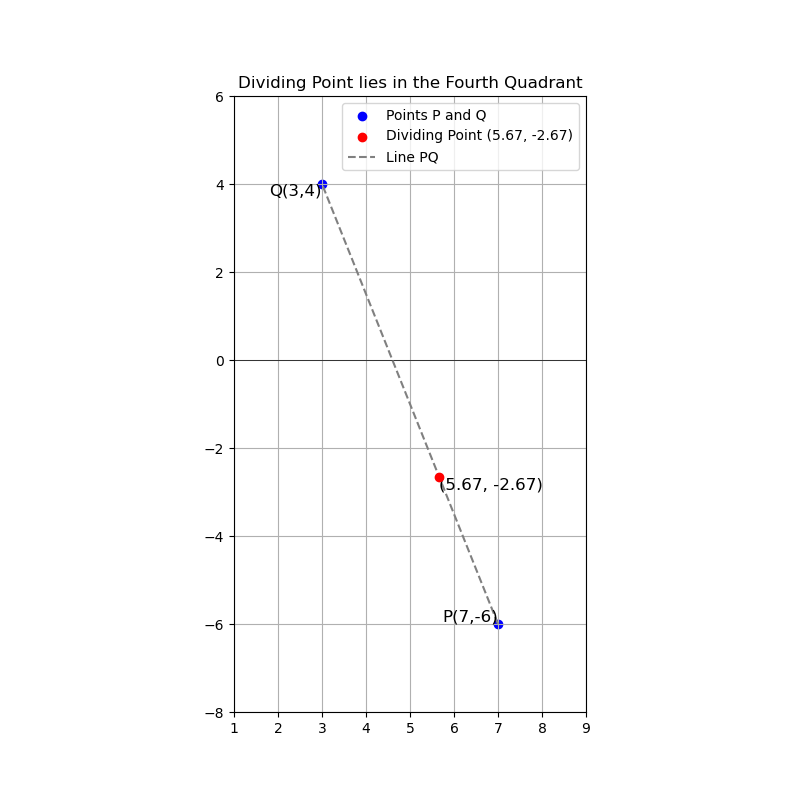
\includegraphics[width=0.7\linewidth]{figs/Plot.png}
			\end{minipage}
			\end{figure}
			
\end{frame}
\section{Codes}
\subsection{C-code}
\begin{frame}[fragile]
\frametitle{C-code}
	C-code shown below is used to find the point $\vec{R}$ and the quadrant in which it lies.
 \lstset{style=Cstyle}
		\begin{lstlisting}
			#include <stdio.h>
#include <stdlib.h>
#include <math.h>
#include "libs/matfun.h"
#include "libs/geofun.h"

// Function to calculate the quadrant based on coordinates
const char* find_quadrant(double x, double y) {
    if (x > 0 && y > 0)
        return "First Quadrant";
    else if (x < 0 && y > 0)
        return "Second Quadrant";
    else if (x < 0 && y < 0)
        return "Third Quadrant";
    else if (x > 0 && y < 0)
        return "Fourth Quadrant";
    else if (x == 0 && y == 0)
    \end{lstlisting}
    \end{frame}
    \begin{frame}[fragile]
    \lstset{style=Cstyle}
    \begin{lstlisting}

        return "Origin";
    else if (x == 0)
        return "Y-Axis";
    else
        return "X-Axis";
}

int main() {
    // Points P (7, -6) and Q (3, 4)
    double x1 = 7, y1 = -6;
    double x2 = 3, y2 = 4;

    // Ratio m1 : m2 = 1 : 2
    double m1 = 1, m2 = 2;

    // Create matrices for P and Q
    int m = 2, n = 1;
    double **P = createMat(m, n);
    double **Q = createMat(m, n);
    P[0][0] = x1;
    
\end{lstlisting}
\end{frame}
    \begin{frame}[fragile]
    \lstset{style=Cstyle}
    \begin{lstlisting}
    
    P[1][0] = y1;
    Q[0][0] = x2;
    Q[1][0] = y2;

    // Calculate the point that divides PQ in the ratio 1:2 using Matadd and Matscale
    double **dividing_point = Matadd(Matscale(P, m, n, m2), Matscale(Q, m, n, m1), m, n);
    dividing_point[0][0] /= (m1 + m2);
    dividing_point[1][0] /= (m1 + m2);

    // Coordinates of the dividing point
    double x = dividing_point[0][0];
    double y = dividing_point[1][0];

    // Find the quadrant
    const char* quadrant = find_quadrant(x, y);

    // Write the result to a text file
    FILE *fptr = fopen("dividing_point.txt", "w");

    \end{lstlisting}
    \end{frame}
    \begin{frame}[fragile]
    \lstset{style=Cstyle}
    \begin{lstlisting}
    if (fptr == NULL) {
        printf("Error opening file!\n");
        return 1;
    }

    fprintf(fptr, "The point that divides the line segment PQ in the ratio 1:2 is: (%lf, %lf)\n", x, y);
    fprintf(fptr, "The point lies in the: %s\n", quadrant);

    fclose(fptr);

    // Free allocated memory
    freeMat(P, m);
    freeMat(Q, m);
    freeMat(dividing_point, m);

    printf("Coordinates and quadrant successfully written to 'dividing_point.txt'\n");

    return 0;
}
\end{lstlisting}


\end{frame}
\subsection{Python code}
\begin{frame}[fragile]
\frametitle{Python code}
Python code reads the point and plots in graph
            \lstset{style=Pythonstyle}
            \begin{lstlisting}
import matplotlib.pyplot as plt

# Function to read the dividing point from the text file
def read_dividing_point(file_path):
    with open(file_path, 'r') as file:
        lines = file.readlines()
        # Extract the coordinates from the first line
        coord_line = lines[0].strip().split(": ")[1]
        x, y = map(float, coord_line.strip("()").split(", "))
        return x, y

# Read the dividing point from the file
dividing_point_file = "dividing_point.txt"
x_div, y_div = read_dividing_point(dividing_point_file)

# Original points P and Q
x1, y1 = 7, -6  # Point P
x2, y2 = 3, 4   # Point Q
\end{lstlisting}
\end{frame}
\begin{frame}[fragile]
\lstset{style=Pythonstyle}
\begin{lstlisting}
# Function to determine the quadrant of the point
def find_quadrant(x, y):
    if x > 0 and y > 0:
        return "First Quadrant"
    elif x < 0 and y > 0:
        return "Second Quadrant"
    elif x < 0 and y < 0:
        return "Third Quadrant"
    elif x > 0 and y < 0:
        return "Fourth Quadrant"
    elif x == 0 and y == 0:
        return "Origin"
    elif x == 0:
        return "Y-Axis"
    else:
        return "X-Axis"

# Determine the quadrant of the dividing point
quadrant = find_quadrant(x_div, y_div)
\end{lstlisting}
\end{frame}
\begin{frame}[fragile]
\lstset{style=Pythonstyle}
\begin{lstlisting}
# Plotting the points and the line segment
plt.figure(figsize=(8, 8))
plt.axhline(0, color='black',linewidth=0.5)
plt.axvline(0, color='black',linewidth=0.5)

# Plot points P and Q
plt.scatter([x1, x2], [y1, y2], color='blue', label='Points P and Q')

# Plot the dividing point
plt.scatter(x_div, y_div, color='red', label=f'Dividing Point ({x_div:.2f}, {y_div:.2f})', zorder=5)

# Draw line PQ
plt.plot([x1, x2], [y1, y2], color='gray', linestyle='--', label='Line PQ')

# Add labels to the points
plt.text(x1, y1, f'P({x1},{y1})', fontsize=12, verticalalignment='bottom', horizontalalignment='right')
\end{lstlisting}
\end{frame}
\begin{frame}[fragile]
\lstset{style=Pythonstyle}
\begin{lstlisting}
plt.text(x2, y2, f'Q({x2},{y2})', fontsize=12, verticalalignment='top', horizontalalignment='right')

plt.text(x_div, y_div, f'({x_div:.2f}, {y_div:.2f})', fontsize=12, verticalalignment='top', horizontalalignment='left')

# Display the quadrant
plt.title(f"Dividing Point lies in the {quadrant}")

# Set the x and y limits
plt.xlim(min(x1, x2, x_div) - 2, max(x1, x2, x_div) + 2)
plt.ylim(min(y1, y2, y_div) - 2, max(y1, y2, y_div) + 2)

# Add grid, legend, and show the plot
plt.grid(True)
plt.legend()
plt.gca().set_aspect('equal', adjustable='box')
plt.show()


            \end{lstlisting}


\end{frame}
\end{document}

